% !TEX root = rapport.tex
\section{Current}
\label{current}
Several input devices in this paper such as the keyboard and the mouse, are still wildely used today but can be seen as historical devices. This is justified by the fact that they remain largely unchanged -- if not in their physical design then in the fashion they are used. On the other hand, a number of other input/output devices that can be seen as recent have a long history behind them. Although \emph{touchpads}, \emph{touchscreens} and \emph{speech recognition} techniques were researched as far back as the 1960's \cite{buxton}\cite{shoebox}, they have only now began to see commercial use and have likely still not reached their "peak". 


\subsection{Touch devices}
Touchscreen devices have become increasingly popular during the last years, following the breakthrough of \emph{smart devices} running specialized operating systems such as Apple's iOS and Google's Android. The technology used in these devices however, have evolved over a much longer time.

One of the first mentions of touchscreens was by E.A. Johnson in 1965, describing a touchscreen and identifying some potential uses in a short article, less than a single page\cite{4205802}. Some of the earliest developed systems came in the beginning of the 1970's. Early prototypes are the PLATO IV\cite{buxton} in 1972, see figure \ref{platoIV}, and a transparant touchscreen was developed and put to use by CERN in 1973\cite{cern}.

\begin{figure}[]
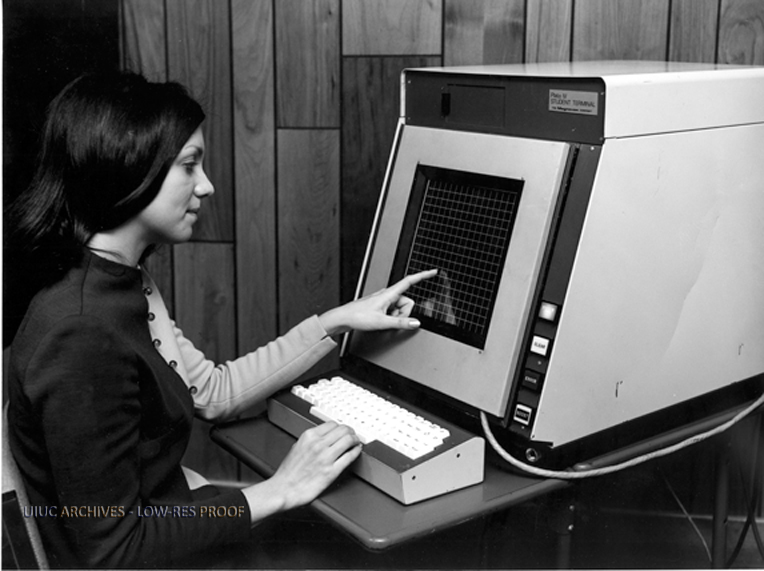
\includegraphics[width=0.8\textwidth] {bilder/platoiv.jpg}
\caption{Student using the PLATO IV.}
\label{platoIV}
\end{figure}
\nocite{platoiv}

The initial uses of touchscreens were point-to-select systems used in for example ATM machines or cash registers in restaurants and were relatively non-demanding on the screen performance\cite{buxton}. There were also early attemps to make \emph{PDAs}\footnote{Personal Digital Assistant}. The first products to enter the market were the Palm Zoomer and the IBM Simon. The Simon was a mobile phone without any physical buttons, having only a touchscreen interface. Beyond regular telephone capabilities, it could also manage information such as a phonebook and be used for drawing and taking notes. Due to this, it is sometimes refered to as the first \emph{smartphone}\cite{buxton}.

Smartphones have seen much development since the release of the Simon, and today it is estimated that more than a billion people use smartphones\cite{billion1}\cite{billion2}. This is largely due to the recent popularisation of the iOS and Android operating systems.

This increase in the number of touch-based devices has changed the way in which we interact with computers, and the new operating systems specifically designed for smartphones have a fundamentally different approach to computer interaction.

The classic WIMP approach requires the user to find the cursor on the display, move it to the desired location and click the mouse button to interact, or use the keyboard to input data. The touch screen on the other hand gives the user the ability to point directly at the desired item at the screen to activate it. An on-screen keyboard appears when it is needed, allowing the computer to show only what is relevant at that point of time. This has made computers so portable that they can be used in almost any context and in a user-friendly way.

One of the big breakthroughs that has allowed the touchscreen to be used as an independent input device by a computer, is the introduction of multi-finger gestures. While early touchscreens could only handle one action (``left mouse button''), the use of multi hand gestures removes the need for buttons. Instead the functionality can be reached by pinching or swiping fingers.

\begin{figure}[]
\includegraphics[width=0.8\textwidth] {bilder/ipadbook.jpg}
\caption{Apple Ipad showing iBooks, with the book Alice's Adventures in Wonderland.}
\label{ibooks}
\end{figure}
% Bild på xerox-musen eller mac-musen
\nocite{ipadbook}

A common application of smart devices is to read e-books. On a traditional computer, the user typically reads the e-book as a document, with all pages following each other from top to bottom. On a \emph{tablet}\footnote{A smart device, typically with a larger screen than a smartphone}, the e-book can be made to look like a book, see figure \ref{ibooks}. The act of swiping a finger from right to left triggers the book to turn the page, similar to what one would do in a physical book. This could be done with another gesture, for example by drawing a circle on the screen or triple-tapping, but these approaches are not as intuitive as the swipe-gesture. This example shows that this type of interaction is not fundamentally more user-friendly, but it \emph{can be} if used in the right way. 

\subsection{Voice recognition}

Voice recognition is another input method that has become increasingly popular in the last years. This input method uses speech recognition by analyzing input from a microphone. Once the spoke word has been analysed, it can be used in several ways.

One ambition is to provide real-time subtitles to spoken text, for example to aid those with hearing disorders. As an input method, the sound input can be parsed by the computer and then trigger a predefined action. This type of speech recognition has recently seen big progress, and is growing in popularity. For example, in the past years Microsoft presented an English to synthesised speech Chinese translator, working in real time and Apple has introduced the \emph{Siri} speech recognition system in their handheld devices.\\

While computers have only recently become powerful and cheap enough to make speech recognition broadly available, its history is much longer. The first working implementation was introduced by Bell Labs in 1952\cite{Davis52}. It could not analyse sentences, instead single words were compared to a small dictionary, the numbers 0 to 9, spoken by a single speaker\cite{juang}. The user was also required to make a small pause between every word for the system to recognize them.

Other systems analysed \emph{phonems}\footnote{Phonemes are the smallest building blocks of the language and consist of the individual sounds used to construct words and sentences} in the spoken text. Early phonem-based techniques could only recognise a subset of phonemes; RCA Labs in 1956 could recognise ten phonemes, spoken by a single speaker, Fry and Denes at the University College in England could recognise 4 wovels and 9 consonants. More notably, they were the first to incorporate statistical information in the analysis\cite{juang}, something that now is fundamental in speech recognition. By analyzing speech at this low level the system becomes less dependant on pauses and dialect in speech.

In the 1980's, the use of \emph{Hidden Markov Models} was introduced in speech recognition\cite{rabiner1986introduction}. The Markov Models use previously gathered statistical data to with some certainty guess which phoneme the user is saying, and the chain of phonemes considered to be correct are then matched to a phoneme-word database to decide which word the user has spoken. The context of the word is also taken into account to prevent homonyms of the desired word to be entered instead. The Markov Model Speech Recognition systems ``learn'' the users voice and speech patterns by using the data from corrections to alter the statistics used to decide which phoneme was spoken.

\begin{figure}[]
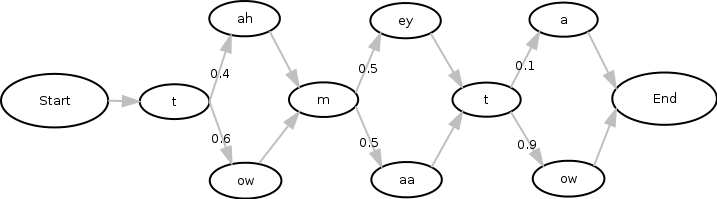
\includegraphics[width=0.8\textwidth] {bilder/tomato.jpg}
\caption{A model describing the statistical values of phoneme input of the word \emph{tomato}. The model contains american and british english pronounciations, with a small statistical favor of the british accent.}
\label{ibooks}
\end{figure}

Most speech recognition software today use Hidden Markov Models for speech analysis\cite{DNN}, but recent research has shifted focus towards the use of a type of artificial neural network, called Deep Neural Networks (DNN). Neural networks have been used for speech recognition since the late 80's\cite{waibel:phoneme}, but the use of DNN is the first that has been shown to have substantial benefits over the use of the traditional markov model approach.

An ongoing research collaboration around DNN exists between the University of Toronto, Microsoft, IBM and Google. Late 2012, Microsoft publicly demonstrated their work with speech recognition -- a system that can translate spoken English into spoken Mandarin in real time and in a voice similar to that of the speaker. In conjunction with the demonstration, Microsofts chief researcher Rick Rashid says about DNNs: ``While still far from perfect, this is the most dramatic change in accuracy since the introduction of hidden Markov modeling in 1979''\cite{chin}.

Speech recognition can be used in many applications. One of these include the the automatic texting of television programs. Another application, which is the main task of the Siri interface, is to respond to short queries by the user, about for example the weather, the current time, web searches and booking systems. This removes the need for the user to interact through a traditional interface, and allows for certain automatisation.